%*******************************************************************************
%****************************** Second Chapter *********************************
%*******************************************************************************

% !TEX root = ../thesis.tex
\zw{Add about how equality does not provide equal outcomes or experiences as the world outside of the model is inherently unjust.}\zw{Mention AAE to introduce the abbreviation}
\chapter{Theoretical Background}\label{chap:socialscience}
In this chapter, we introduce core concepts from social science that we employ in this thesis. This will serve as foundational knowledge for what we interpret as abusive language and hate speech. Subsequently, a consideration of multiple of these may be necessary to determine if speech is derogatory and will inform our recommended solution for handling such speech. Additionally, we seek to introduce how we will use these concepts in the thesis.

\section{Abuse}
Considering the typology proposed in \cite{Waseem:2017} (see Table \ref{tab:typology}), we see multiple ways abuse can be expressed along the axis of directed, generalized, explicit, and implicit abuse. As we briefly touched upon in Chapter \ref{chap:intro}, we will only be considering directed abuse that is either implicit or explicit. While the examples in Table \ref{tab:typology} may seem very straightforward in their abusiveness, it is important to note that this is not always the case. For instance in the case of the n-word and other slurs exist in a context of the societal structures. One very clear illustration of the impact of societal structures is the n-word and are the different connotations depending on context, speaker, and listener. Should a non-black person use the n-word, it speaks into the context of the forced subjugation of black people. However, when black people use it within the context of black communities, it lends itself to a history of solidarity in face of subjugation \citep{Rahman:2011}. Therefore, it is necessary to consider the concepts {\it privilege} of the ruling groups and {\it oppression} of the subjugated groups to inform our understanding of abuse.

\begin{table*}[ht]
\centering
\begin{tabular}{p{\textwidth/30}|p{0.45\textwidth}|p{0.45\textwidth}}
  & \textit{Explicit}    & \textit{Implicit} \\\hline
    \multirow{4}{*}{\rotatebox[origin=c]{90}{\textit{Directed}}}    &   {\scriptsize``Go kill yourself'',  ``You're a sad little f*ck'' \citep{Hee:2015a}}, \newline {\scriptsize ``@User shut yo beaner ass up sp*c and hop your f*ggot ass back across the border little n*gga''  \citep{Davidson:2017}}, \newline {\scriptsize ``Youre one of the ugliest b*tches Ive ever fucking seen'' \citep{Kontostathis:2013}}. & {\scriptsize ``Hey Brendan, you look gorgeous today. What beauty salon did you visit?'' \citep{dinakar2012common}, \newline ``(((@User))) and what is your job?  Writing cuck articles and slurping Google balls?  \#Dumbgoogles'' \citep{Hine:2016},\newline  ``you're intelligence is so breathtaking!!!!!!'' \citep{dinakar2011modeling}}\\\hline
  \multirow{5}{*}{\rotatebox[origin=c]{90}{\textit{Generalized}}} & {\scriptsize``I am surprised they reported on this crap who cares about another dead n*gger?'', ``300 missiles are cool! Love to see um launched into Tel Aviv! Kill all the g*ys there!'' \citep{Nobata:2016}, \newline ``So an 11 year old n*gger girl killed herself over my tweets? \^ \_ \^\ thats another n*gger off the streets!!'' \citep{Kwok:2013}}. & {\scriptsize``Totally fed up with the way this country has turned into a haven for terrorists. Send them all back home.'' \citep{burnap2015cyber}, \newline ``Gas the skypes'' \citep{magu2017detecting}, \newline ``most of them come north and are good at just mowing lawns'' \citep{dinakar2011modeling}} \\
\end{tabular}
  \caption{Typology of abusive language \citep{Waseem:2017}.}
\label{tab:typology}
\end{table*}

\section{Privilege}\label{sec:privilege}
The concept of privilege was first introduced by \cite{Dubois:1935} as ``psychological wage'' in his work ``Black Reconstruction in America''. In this work he describes a deliberate effort to segregate poor whites and blacks to prevent potential alliances between the two. He argued that efforts were made to distinguish working class whites along racial lines by aligning them with their employers. The consequence of this being that working class whites came to feel a superiority over blacks. 

Since this early exploration of psychological wage, or its' more current term: ``privilege'' a great deal of work has been done exploring the psychological and social differences along racial hierarchies. Further, the concept of privilege has been applied to the concepts of gender \citep{Beauvoir:1953,Butler:1990}, race \citep{Crenshaw:1989,Dubois:1935}, sexuality \citep{Foucault:1978}, religion \citep{Beaman:2003}, and other aspects of identity. One notable work, that we will rely heavily on in this thesis is \cite{McIntosh:1988}, in which they explore the differences in privileges afforded along gender and racial lines in her own life. Specifically, she explores the privileges that are afforded to men, but not to her due to her gender; and privileges that are afforded to her due to her whiteness but not afforded to black women.\vspace{5mm}

In more concrete and operationalizable terms, the concept of privilege seeks to describe that some demographics receive beneficial treatment due to their identities or \textit{intersection} of identities, i.e. gender, race, religion, sexual orientation, and mental health. Many social issues have been explained through the concept of privilege such as gender representations \citep{Butler:1990}, rights for homosexual couples \citep{Foucault:1978}, and police treatment of black people in the United States of America \citep{Voigt:2017}. 

In recent years, there has been a greater focus on social and economic disparities, including not being financially punished for ones gender expression \citep{Lombardi:2002}; and the increased risk of lethal encounters with law enforcement depending on racial identity \citep{Zack:2015}.

\section{Oppression}\label{sec:oppression}
When speaking of privilege it is necessary to also consider its counter-part: Oppression. Oppression, in the frame of privilege, refers to the (continued) marginalization of demographics as compared to the privileged groups \citep{Abberley:1987}. Oppression can thus range from the systematic underpayment of women and trans people \citep{Lombardi:2002,Pew:2018}, to the underrepresentation of people of color in popular media \citep{Dixon:2006}, to the ability to move safely in public spaces \citep{Valentine:1989}. 

It is crucial to note that not all marginalization is oppression \citep{Abberley:1987}. For instance, should a white man in the United States of America feel unsafe around men of color, this does not amount to oppression. While there may be singular instances of feeling unsafe, these instances do not translate to a wider collective experience of their demographic. As an example, a white man may experience police brutality at the hands of black police officer, however police brutality and unjust treatment of white men is not a in institutional problem that afflicts most, or even many white men. In comparison, should a black man experience police brutality at the hands of a white police officer, this speaks into a wider history and culture of black men being abused by the police. As such the institutional power that the white and black police officer wield, respectively, speak to two different societal positions and histories of oppression. 

However, these imbalances in power do not only occur in physical settings, they also occur in spoken and written word. Consider for instance the case of coded language such as the term ``thug''. While people of all creeds may use the term, the connotation that occurs with many people is specifically an African American man, due to representation in popular media \citep{Dixon:2006}. Thus, while ``thug'' may be used to refer to a person of any race or gender, the use of the term by politicians invokes a specific imagery. 
Another such example is with regard to terrorism. In many cases, terrorist acts perpetrated by white people are attributed to insanity, frustration, and many other reason \citep{Powell:2011}. However, considering narrative surrounding similar acts perpetrated by brown men, a very different picture arises; one that speaks to terrorist acts and often linked to religious fanaticism, regardless of the piety of the suspect in question.

As we are alluding to, power and privilege are closely related, such that a group which holds institutional power cannot be oppressed on the axis of the intersection where the group is in power \citep{Eisenstein:1977}. 

% When speaking of privilege, it is necessary to also consider its inverse: Oppression. Oppression refers to the marginalisation of demographics as compared to the privileged groups \citep{Abberley:1987}.\av{make explicit why the inverse relation} Thus it refers to the systematic underpayment of women and trans people, the under-representation of people of colour in popular media, the ability to safely move in public spaces. It is crucial to note that while regardless of their identities may experience not feeling safe in a public place, it is not oppression unless one feels exposed due to their demography and that this feeling of not being safe is a common feeling within the demography due to the structural position of the demography in society \citep{Abberley:1987}.\av{rephrase} In addition, oppression and power are closely related, such that a group in power cannot be oppressed (on the axis of the intersection where the group is in power) \citep{Eisenstein:1977}. E.g. A insurance premium for private healthcare is not necessarily oppressive even though it targets people with high incomes as their disposable income allows for such taxation. Conversely, high insurance premiums, when no low-cost public insurance is available, may be oppressive as it prevents access to healthcare for people with little disposable income.\av{don't see where the power comes into play. Also better to have definite examples}

% \section{Micro-aggressions}\label{sec:micro-aggression}
% The concept of micro-aggressions was first introduced by \cite{Pierce:1977} in the field of psychology, in an examination of the influences of TV commercials. The concept seeks to describe the many situations where discriminative aggression is not necessarily the intent, and as a single instance it is an extremely small and insignificant. However, given the sheer number of them that oppressed people are confronted with, they injure and force an otherness upon peoples of oppressed minorities. 
%
%
% \cite{nadal:2011} appropriately referred to micro-aggressions as 'death by a thousand cuts'. Instances of micro-aggressions can be the insistence of asking racialised minorities where they are from and following up with 'where are you \emph{really} from?' As this becomes an insistence that they do not hail from the place that they have told you \citep{Sue:2007}. Micro-aggressions, while at times unconscious on the part of the person uttering them, often serve to accentuate difference, e.g. ``I believe the most qualified person should get the job, regardless of race'' \citep{Sue:2007}. Here suggesting that race is not normally an issue, however that race may influence such that the most competent person is not offered the job. While this may sound reasonable, it is very rarely brought up in the case of a white person getting a job (in the western hemisphere) but often pointed out when a person of colour receives the job offer. While seemingly innocuous, it becomes an argument against diversity and inclusion policies that may be instituted to account for a lack of diversity in a given organisation.
% Recently a Google employee, at the time wrote a brief arguing against gender diversity policies in part arguing that the better candidates should be employed rather than attempting to improve upon disparities in gender representation at the company.
%
%
% Micro-aggressions can also serve to neglect and undercut different realities \citep{Sue:2007}, e.g., ``I don't see race''. In this case the speaker diminishes and invalidates that there are different realities based on race and that these realities can lead to vastly different opportunities in life. Similarly to the previous paragraph this statement may seem innocent at initial glance, however upon further inspection becomes quite problematic. In this case, the claim ``I do not see race'' ends as a way to also state that they do not see nor wish to see the experiences racial expressions bring with them, nor do they see the mistreatment by governmental bodies. It thus becomes not just well intended denial of racial influences that everyone is marked by, it becomes a denial of reality of the person whose very existence is constant subject to consequences and prejudice that stem from having a body of colour.
% Finally, \cite{Sue:2007} also argue for a third category, something they call micro-assaults. Micro-assaults are closer to traditional, overt racism in the use of terms such as ``oriental'', ``coloured'', or discouraging interracial interactions and relationships. While these terms are offensive, they are not explicitly offensive as some slurs are, however they suggest a racial hierarchy in the use of slightly offensive terms. Similarly, discouraging interracial interaction and relationships speak to understanding a racial hierarchy where interaction with other races is seen as sinking to a lower level.
%
% \zw{Rephrase, there's a word for this.}
%
% \cite{Donald:2014} and \cite{Thomas:2008} argue against micro-aggression suggesting that they are trivial cases of racism and should be ignored. In employing this argument, they neglect that the impact of micro-aggressions are exactly from the compound effect leading to further marginalisation \citep{Pierce:1977}. Further, \cite{Thomas:2008} argue that considering micro-aggressions as transgressions will have adverse effects on free speech and interracial interaction
%
% % \begin{aquote}{\cite{Pierce:1977}}
% %   These are subtle, stunning, often automatic, and non-verbal exchanges which are ``put downs'' of blacks by offenders. The offensive mechanisms used against blacks often are innocuous. \emph{The cumulative weight of their never-ending burden is the major ingredient in black-white interactions}. This accounts for a near inevitable perceptual clash between blacks and whites in regard to how a matter is described as well as the emotional charge involved.
% % \end{aquote}
%
% % \cite{Thomas:2008} also argue that the effects of considering micro-aggressions as transgressions will have adverse affects: \av{doesn't follow from the previous sentence}
% % and that they may influence a desire to associate with marginalised people:
%
% \begin{aquote}{\cite{Thomas:2008}}
% [micro-aggressions] could have a chilling effect on free speech and on the willingness of White people, including some psychologists, to interact with people of colour.
% \end{aquote}
%
% As such \cite{Thomas:2008} argues against a use of the theory of intersectionality, not so much on the merits or correctness of the theory, but rather on the grounds that it will further complicate interracial relations. \cite{Thomas:2008} suggest that rather than white people correcting their behaviour as to not transgress upon black people; people of colour should accept these transgressions such that there are fewer breaches in communication.
%
% Furthermore, \cite{Thomas:2008} argue that the need one may have to confirm a microaggression, given its subtle nature, invalidates that it is racist. To \cite{Thomas:2008} an event of racism is always unambiguous. However, this suggests that all racism, and by extension all microaggressions, are overt. Thus failing to account for the subconscious nature of biases, their expressions, and that marginalised communities learn the same biases but often unlearn them through exposure to their own communities.
%
% % Considering the implications of the statement by \cite{Thomas:2008}, \cite{Thomas:2008} seek to invalidate the theory based on its effects rather than the correctness of the theory.
% % Furthermore, \cite{Thomas:2008} suggest that the potential need for validation of the offence in a racist incident (as shown in \cite{Sue:2007}) invariably means that the incident is not racist.\av{I don't get this} This suggests that all racism, and by extension all micro-aggressions, are overt. This argument however fails to take into account the often subconscious nature of biases, their expression, and that marginalised minorities may themselves have learned the same biases.

\section{Intersectionality}\label{sec:intersectionality}

In this PhD, we will apply an intersectional approach to analyze biases. Intersectionality is a theoretical framework founded by \cite{Crenshaw:1989}, the framework seeks to describe how multiple identities can intersect with one another to create unique forms of oppression, e.g. the oppression faced by black homosexual people is different than those faced by straight black people and by homosexual white people. \cite{Crenshaw:1989} argues that one cannot separate one identity from another, and that ``the intersectional experience is greater than the sum of racism and sexism''.

A compelling and clear case of different identities intersecting and influencing is the wage gap in the United States of America, where there are significant differences between income between black and white women as well as women compared to men \citep{Neal:2004}.

The justification and need for an intersectional framework for analyzing and dealing with oppression is further made clear in the case of Moore v. Hughes Helicopter \citep{Crenshaw:1989}. In this lawsuit Moore, a black woman was not allowed to represent a class of other black women that had been bypassed for promotions due to the fact that neither black men nor white women were discriminated against. \cite{Crenshaw:1989} argues that the most likely interpretation of this decision to deny the class is that not all women were discriminated against and not all black people were discriminated against, only black women and as such Moore could not represent a class of women or black people. Thus, the court ruled that black women, in spite of facing discrimination based on the combination of race and gender, could not constitute their own class with regard to discrimination that only affected them.

Beyond the case of black women, the intersectional framework presented by \cite{Crenshaw:1989} has proven useful in applications to sexual orientation, sex work, HIV infected persons \citep{Logie:2011}, and other oppressed classes \citep{Erevelles:2010}. Furthermore, \cite{Verloo:2006} analyzed the application of intersectionality, or the lack thereof in European Union policies addressing discrimination. In a Natural Language Processing context, \cite{Waseem-Hovy:2016} and \cite{Waseem:2016} apply research from gender studies and critical race theory to devise their annotation guidelines and their analysis of hate speech.

Intersectionality allows for insight into things that cannot be the object of legislation for instance, seeing members of ones own race in media, speaking time at academic events, and not having to educate their children on systemic racism for the children's physical safety \citep{McIntosh:1988}. The framework also allows for insight into discrimination that can be legislated against, such as the Moore V. Hughes Helicopter case \citep{Crenshaw:1989}.

\section{Pseudonymity and Anonymity in Social Media}\label{sec:pseudonymity}

As this Ph.D. will deal with data published by individuals who may not be public figures, it is necessary to consider the topic of anonymity and pseudonymity on social media platforms.

Previous research on anonymity has considered anonymity as a spectrum \citep{Qian:2007,Donath:1999}, going from the completely anonymous to fully named. On the other hand, \cite{Nagel:2015} considers anonymity a more complex space, inhabited by pseudonyms, mononyms, stage names, and usernames amongst others. Proponents of named social media sites argue that anonymity encourages anti-social behavior \citep{Galperin:2011}. On the other hand \cite{Nagel:2015}, find this argument misunderstands privacy and identity in both online and offline spaces. \cite{Nagel:2015} argue that identity is enacted with territorial and contextual boundaries in the offline world, i.e. experiences shared with ones family may differ from those shared with friends, boundaries that are removed in the online world as users interact with their entire social circle, in what \cite{Marwick:2011} refer to as context-collapse. \cite{Nagel:2015} suggest that the use of pseudo- and anonymity online can function in a similar fashion to the territorial and contextual boundaries found in the offline world. 

To examine how anonymity and pseudonymity is constructed and how it influences, \cite{Nagel:2015} and \cite{Nagel:2013} consider identity on Reddit, a social media site with forums in which users, who are hidden usernames (which may or may not bear reference to their real name) can post and vote on content. Specifically, the forum \cite{Nagel:2013,Nagel:2015} consider is ``Gonewild'', a forum which describes itself as ``an amateur exhibitionist community'' \citep{Nagel:2015}. On Gonewild, users post nude and semi-nude pictures of themselves, however their faces and names are very rarely associated with these posts. In fact, the forum offers guidelines for ensuring safety when posting images:

\begin{aquote}{\cite{Nagel:2013}}
The internet is a public place. You are posting naked pictures of yourself on the internet[$\ldots$] If you want to be as anonymous as possible, take the following precautions.
1. Make a throwaway reddit account.

2. Don't include your face in your photos. If you must, blur or blackout your features.

3. Take pictures against difficult-to-identify backgrounds. Plain walls or colours work well. 
\end{aquote}

\cite{Nagel:2013} consider the technological and cultural codes that afford anonymity on Gonewild and the risks of posting sensitive information online in an effort to highlight the importance of nuanced understandings of anonymity online. \cite{Nagel:2013} argue that anonymity plays a crucial role in online communication, as a way for users to segment and limit their audience according to what they aim to share, i.e. many users on Gonewild create throwaway accounts to limit the risk of other reddit users undermining their credibility because they posted on Gonewild:

\begin{aquote}{\cite{Nagel:2013}}
Such attention, when unwanted, can prompt users to disguise themselves on reddit by creating a ``throwaway'' account.
\end{aquote}

By creating such throwaway, pseudonymous accounts they are afforded the ability to express their sexual selves in while retaining a disconnect with the rest of their online and offline lives without compromising their ability to interact with their audience or face negative repercussions \citep{Nagel:2015}.\vspace{5mm}

\noindent With the recent implementation of the General Data Protection Regulation, ensuring anonymity has become more strict than with the DPA. For this reason, we will pseudo-anonymize all users by replacing usernames with a hash and placing all user information in encrypted files, on encrypted disks. User information can thus only be obtained with a key and further obtaining the user hash. Due to the impact of the speaker and listener contexts, it is not possible to entirely anonymize the data sets at this point. It is our intention to fully anonymize the data sets at the earliest possible point, and only use user information if no other option is available.

% \subsection{Anonymity}
% The method that allows for most freedom and safety for users is to fully anonymise data collected on social media. However, due to the phrasing of anonymity in the DPA, which states that a user may not be recoverable obtaining full anonymity on social media data sets is impossible should one seek to work on a user level. In some experiments, namely author profiling, it will not be possible to abstract away from the user level initially. For this reason, at an early stage in our research, it will not be possible to anonymise the data sets fully. 
%
% It is our intention to fully anonymise our data sets at the earliest possible point, however, this point will not occur until author profiling tools have been built, such that they can be used in subsequent research. In all subsequent research on social media data, a partial anonymisation will be performed prior to obtaining demographic information by using the author profiling tools. Once the demographic information of a user has been obtained a random hashstring will be generated to identify the user and all user information beyond the demographic knowledge will be dropped. For the sake of reproducibility, a key mapping between user ID's and hashstrings will be stored on a different passport protected encrypted device thus ensuring that the requirements of the DPA are fulfilled.

\section{Moderation Practices}
To understand how moderation can work, it is necessary to consider the communicative power of reporting frameworks. In \cite{Crawford:2016}, the analysis of frameworks for reporting is motivated by the fact that reporting content is a method for users to communicate with the platforms. As flags become communicative devices for the users of a site to convey the desired values of the community \citep{Crawford:2016}. At the same time, flagging allows for a company to specifically control the expressiveness of the communication between users and the company and the volume of this communication \citep{Crawford:2016}. Volume can be controlled by the ease of access to flagging documents and expressiveness can be controlled by the level of detail users can provide when reporting. \cite{Crawford:2016} argue that a low expressiveness can lead to posts that are reported for a distinct number of reasons can be conflated with one another, if only a few options are available. In addition, a lack of options when flagging can communicate that the company is not interested in distinguishing what users find unacceptable, they simply wish to know that some content is deemed unacceptable byt the community but not why \citep{Crawford:2016}.

Oftentimes, flagging is a solitary effort, where single users will communicate that they find content unacceptable, such as when an image of two male actors kissing on the TV show EastEnders was uploaded to Facebook. This image received a great number of reports stating it as sexually graphic and was subsequently removed. Once removed, it created a great deal of outrage as Facebook were accused of homophobia and hypocrisy as images of gay couples kissing were being flagged and removed while images of straight couples kissing were not. Following this controversy, Facebook undid their removal of the image and apologized for removing it \citep{Crawford:2016}.
Considering flags as a communicative device allows for flagging as a strategic means of communication for users to further an agenda. For instance, a group of bloggers angered by the pro-Muslim content on YouTube started ``Operation Smackdown'' which was launched in 2007 and was active up until 2011. In Operation Smackdown, the bloggers coordinated their supporters to flag certain YouTube videos under the category of ``promotes terrorism''. In this coordinated effort, the bloggers created instructions for flagging and created playlists of videos they wanted to targeted that day. They also created a Twitter feed announcing the videos to be flagged. The bloggers would celebrate removed videos and attack YouTube and Google for letting others remain \citep{Crawford:2016}. These flags can be considered as coordinated attacks which can be perpetrated by a group against both minorities and majorities alike.

\section{Safety}\label{sec:ethics:safety}
Given that the topic of thesis may touch upon some very sensitive issues, such as gender and racial biases, it is necessary to ensure the safety of participants and researchers involved. Given that much of the controversial data will be personal data, this safety is largely ensured by following the Data Protection Act (DPA) and the General Data Protection Regulation (GDPR) through their focus on ensuring that un-anonymized participant data is only available to the researchers working on the project. Indeed, the DPA suggests that data is anonymized at the earliest possible step, and that it is stored on encrypted drives such that participant, and in extension researcher safety is ensured.

In this project, there will be a need for retaining un-anonymized data sets in regards to determining the speaker and listener demographics. To ensure participant safety, we will ensure that any data sets that have not been released publicly are stored in encrypted folders, and encrypted devices where possible. In addition, access to the data will be restricted to the active researchers in the project and potentially the respective supervisors.

\section{Participant Agency and Informed Consent}
At this point, the requirements of the GDPR for consent in social media research is not entirely clear to us. We will follow the requirements of the GDPR and update this once we have a clear understanding of how and if consent will be required.
% The social media aspects of this project calls for unobtrusive observation on social media, it is not possible to conduct the research while obtaining informed consent from the users. Rather, we approximate consent by publication. Given the public nature of Twitter, which will be our primary if not only source of social media data, we argue that users are aware of their tweets being published to the world, in addition, should users frequently use ``hashtags'', a method for categorising and widening the audience of tweets, it implies that not only are they aware of the public nature of Twitter, they are explicitly seeking to widen the audience of their tweets to a global scope. In our project, we will collect tweets using hashtags and the tweets users of those hashtags publish. In order to ensure that the users are aware and explicitly utilise the public nature of Twitter, we will not use tweets from users that use hashtags less than at a given ratio\footnote{We need to determine this ratio based on real use of Twitter.}
%
% To ensure user agency, we will remove tweets that are deleted and we will only collect tweets from public accounts.

\section{The Legality of Abuse}

As the detection of abuse may be closely linked to the content moderation and the removal of content, any consideration of tools with the purpose of identifying abuse must also consider the legal context context in which they may operate. In this we consider two forms of legal contexts: regulatory frameworks and platform policies and their influences on using automated methods for detecting abusive language.

\subsection{Platform Policies}

Many large social media companies lay out their policies for acceptable behaviour on their platforms, often detailed in their user guidelines. Many of these have similar phrasing on the acceptance of abusive language,\footnote{For the full policies see \url{https://en-gb.facebook.com/communitystandards/hate_speech} for Facebook's policy on hate speech, \url{https://help.twitter.com/en/rules-and-policies/hateful-conduct-policy} for Twitter's policy on hate speech, and \url{https://www.redditinc.com/policies/content-policy} for Reddit's policy on prohbited content.} in \autoref{fig:policies} we show excerpts of the policies on hate speech and prohibited content of three social media platforms.

\begin{figure}[!htb]
  \begin{minipage}{0.32\textwidth}
    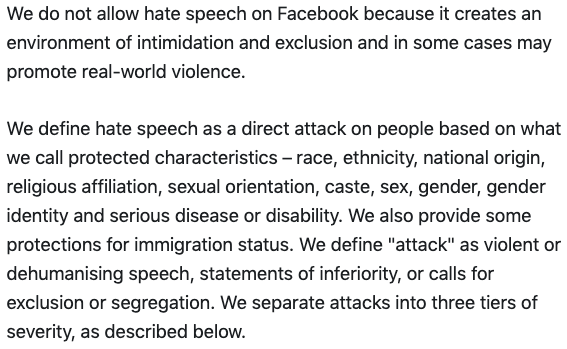
\includegraphics[width=\linewidth]{Chapter2/Figs/Facebook.png}
    \caption*{(a) Facebook}
  \end{minipage}\hfill
  \begin{minipage}{0.32\textwidth}
    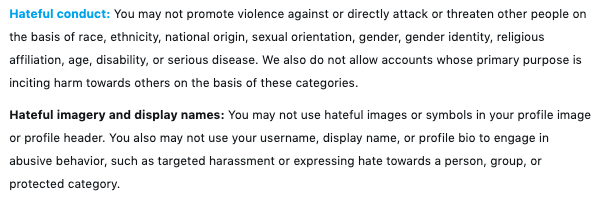
\includegraphics[width=\linewidth]{Chapter2/Figs/Twitter.png}
    \caption*{(b) Twitter}
  \end{minipage}\hfill
  \begin{minipage}{0.32\textwidth}
    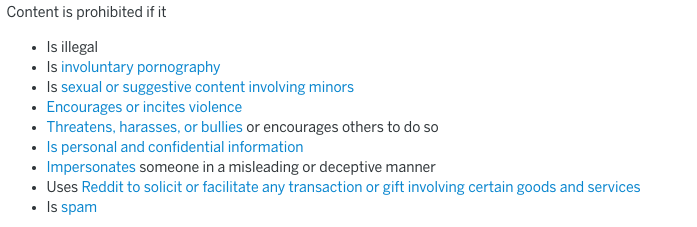
\includegraphics[width=\linewidth]{Chapter2/Figs/Reddit.png}
    \caption*{(c) Reddit}
  \end{minipage}\hfill
  \caption{Excerpts of policy on prohibited content and hate speech from Facebook, Twitter, and Reddit.}
  \label{fig:policies}
\end{figure}

In all three excerpts of the policies, we see a prohibition of content which attacks others, Reddit's policy on encouraging and inciting violence they further outline that users should not post content that\footnote{for the full policy see \url{https://www.reddithelp.com/en/categories/rules-reporting/account-and-community-restrictions/do-not-post-violent-content}}

\begin{quote}
  [\dots] that encourages, glorifies, incites, or calls for violence or physical harm against an individual or a group of people
\end{quote}

establishing similar outlines for acceptable conduct as seen on Twitter and Facebook. Facebook note in their Community Standards Enforcement Report\footnote{See report here: \url{https://transparency.facebook.com/community-standards-enforcement\#hate-speech}} that they acted on $4$ million items for hate speech and $2.8$ million items for bullying and harassment in the period of January to March 2019. The report does not detail the number of user reports received, nor the amount of content which was not removed.\footnote{Acted on here means acknowledging that the content does violate community standards yet and an action was taken by Facebook.} Considering the scale of the items which have actions taken for different kinds of abuse, there is an incentive to automate allow for some automation to guide the attentions of human moderators or decrease the number items which moderators need to consider.\footnote{The Community Standards Enforcement Report details that automated systems are deployed but do not detail the performances of the system in terms of accuracy, precision, or recall.}

While Facebook report high numbers of removals, the performance of their (human and automated) moderation practices have been the source of criticism as a number of activists have reported being temporarily banned for speaking about racial discrimination while abuse and discrimination received is not addressed \citep{Sharif:2019} and common users noting that simply talking about race may mean that your post is removed, particularly if the poster is not white \citep{Guynn:2019}. A report from Propublica details that the policies of Facebook in determining whether a post violates community guidelines, by seeking global standards, effectively ``protect the people who least need it and take it away from those who really need it.''\citep{Angwin:2017}

%In fact, automated processes are used for $14.1\%$ of actioned content for harassment and bullying and $64.4\%$ for hate speech. Considering then the number of appeals, for hate speech more than $1$ millioned actioned items were appealed, and $496$ thousand were appealed for bullying and harassment. Numbers are not provided for the precision of the automated systems.

\subsection{Regulation} \zw{Limit the length of this as this will be less prominent in the thesis}
In recent years several different governments have sought to address the issue of online abuse, for isntance the British Home Office \citep{HomeOffice:2016} and the European Commission \citep{EUCommission:2016} gave guidelines and a call to action to social media networks. In a different approach, the German government passed the Network Enforcement Act (NetzDG) \citep{NetzDG:2017} in an aim to provide regulation to curb online abuse and misinformation. The regulation states that online platforms will face fines if they systematically fail to remove hate speech within $24$ hours.\vspace{5mm}

Building on this, the European Union is currently considering regulation on disseminating terrorist content which may have implications on hate speech and how social media platforms deal with issues such as hate speech \citep{EUCommission:2018} through the difficulty in distinguishing between content which promotes terrorism and content which is simply hateful - a consideration which is highlighted in the response from the European Union Agency for Fundemental Rights (FRA). In their opinion, the FRA suggest that the proposed regulation should provide a clear definition of terrorist content which limits it to inciting or promoting terrorist activities or providing instructions on the making or use of weapons \citep{FRA:2019}. A key point of the regulation states that the platforms must remove content within $1$ hour of receiving notice from a trusted authority.\vspace{5mm}

More severely, two bills on sex trafficking were passed in the United States of America, namely the Stop Enabling Sex Traffickers Act (SESTA) and the Fight Online Sex Trafficking Act (FOSTA). These two bills aim to prevent sex trafficking by removing sexual solicitation online. While the critiques of the bills are numerous for flaws in their conceptualisations \citep{Romano:2018}, impact on criminal investigative work \citep{Q:2018} and the consequences for sex workers - including missing persons and deaths of sex workers \citep{Blue:2018,Simon:2018}, the implications of the bills are far greater in three espects:

\begin{enumerate}
  \item{The bills weaken \citep{Romano:2018,Stryker:2018} in Section 230 of the Communications Decency Act (CDA) - which holds that computer service providers are not publishers and thus not liable for content on the platform \citep{EFF:230},}
  \item{the bills are effective retroactively \citep{Stryker:2018}, therefore necessitating moderation of both new and historic content, and}
  \item{the bills do not require a request to remove content prior to potential consequences for not upholding the laws.}
\end{enumerate}

While the weakening of Section 230 of the CDA falls in line with the European and German regulations by holding social media companies accountable for the content on their platforms, the European and German initiatives require are designed such that social media platforms respond to flagging and requests for content removal. Furthermore they are not in effect retroactively. These differences strongly encourage the use of machine learning to be applied regardless of the precision of the systems.\vspace{5mm}

\subsection{Court Cases}  \zw{Limit the length of this as this will be less prominent in the thesis}

Considering pressures to turn to automation, it is relevant to consider the class action lawsuit against Facebook\footnote{see Scola v. Facebook, Inc and Pro Unliminted, Inc., 2018, Civil Action No.: CIV0513} and the lawsuit Microsoft\footnote{See Soto and Blauert v. Microsoft, 2017, Case No.: 16-2-31049-4} by former content moderators from each company. Both lawsuits will be going forward and have not been settled. In both lawsuits, the plaintiffs report that they suffer from Post-Traumatic Stress Disorder as a result of being exposed to content such as beheadings and child pornography coupled with insufficient support and debriefing opportunities.

\subsection{Collective Pressures}

In the previous subsections we outline different three different pressures for content moderation on social media companies: Regulatory pressure, legal pressures, and pressures of volume. These pressures collectively generate a strong motive for deploying automated systems for content moderation including identifying abuse and hate speech. Considering however the issue of abuse, often context is required. However, while there may be an strong desire for automated systems, the issues in the impact on marginalized people highlight that uniform rules to apply to all groups may in fact effectively be discriminatory, which calls for systems to be developed thoughtfully with the knowledge that they may be discriminatory.

% TODO Look at this again later. It doesn't fit here. \cite{banks:2010} suggest that the lack of accountability, the immediacy, and global nature of the internet has allowed for it to become ``an ideal tool for extremists and hate mongers to promote hate''. In addition, it was the hopes of Facebook that increased accountability would lead to a decrease in hate speech \citep{Levine:2013}.

{\color{red}
\section{Situated knowledge and subjugated data discourses} \zw{Actually write this as previous work instead of what we're going to do}
Finally, one cannot talk about data in the context of machine learning without considering where it comes from or how the methods applied to it will affect it. We borrow here loosely from \cite{Fraser:1989} and \cite{Spivak}'s notion of the ``subaltern counterpublics'', that is ``parallel discursive arenas where members of subordinated social groups invent counterdiscourse, and Foucault's notion of dominant and subjugated discourses to understand the processes of marginalisation occurring through the use of machine learning models. Similarly, we rely on \cite{Haraway:1988}'s work on ``Situated Knowledge'' to better understand how machine learning methods, and data used in such methods assume a ``view from nowhere'', employing the ``God trick'' allowing for the illusion of objectivity as a result of applying mathematical modelling to data.

\cite{Harway:1988,Gitelman:2013,Gitelman-Jackson:2013,Mohanty:1984}

\section{Theoretical Approaches to Content Moderation}

\zw{Add page numbers to the quotes, once your physical copy of the book arrives.}
In her work on theories of social pollution, Mary Douglas \citeyear{Douglas:1966} examines how meaning and community are made through the positive reordering of the environment to separate the subjects and objects that belong and those that do not, i.e. what is not and what is dirt. She argues that `dirt is the by-product of a systematic ordering and classification of matter, in so far as ordering involves rejecting inappropriate elements' \cite{Douglas:1966}. Dirt is then not an independent attribute of an object or subject, but a `residual category rejected from our normal scheme of classifications' \cite{Douglas:1966}. This classification between what is dirt and what is not, practised through rituals and habits that create coherence within communities, helps establish borders between what and who belongs in a group and what does not. As communities reject the impure, members of the collective, or in fact society, form a shared meaning. Through these processes of meaning-making, or border hygiene the collective can maintain its integrity. Dirt then becomes something communities avoid in order to prevent the breakdown of meanings, and by extension the community itself.

To \citet{Douglas:1966} the avoidance and removal of dirt are not negative processes of removal, they are a `positive effort to organize the environment' \cite{Douglas:1966} of the community in which the removals takes place. Further she argues that we seek to re-order our environment to make it conform to an idea.

As the identification, demarcation, and expulsion of dirt are collective actions, the definitions and understandings of what constitutes dirt is a subjective in nature and meaning can only be attributed within a given system: `no single item is dirty apart from a particular system of classification in which it does not fit' \cite{Douglas:1966}. Further, in her conceptualisation dirt is an encompassing label for `all events which blur, smudge, contradict or otherwise confuse accepted definitions' \cite{Douglas:1966}. Dirt is then contextual, and what is dirty in one situation may not be dirty in another. She exemplifies this through the mundane: food is not necessarily dirty, `but it is dirty to leave cooking utensils in the bedroom' \cite{Douglas:1966}.

Given the contextual nature of dirt, many might imagine that they are unequivocally able to identify dirt, \citet{Douglas:1966} argues that detecting dirt is complex as with the contextual nature of dirt, it follows that there can be no such thing as absolute dirt or clean, as these depend on the subject observing it. Thus, what is dirt to one might be valuable to another. Conversely, as \citet{Lepawsky:2019} argues, the positionality of discarding, or cleaning, may result in discarding or maintaining things that are valuable to one, but are harmful to another. Who then gets to exert such power to determine what stays and what remains becomes a question of differential power relations. Indeed, \cite{Hall:1993} similarly ties the classification of dirt and the clean to racist logics of social purification:

\begin{quote}
  What you do with dirt in the bedroom is you cleanse it, you sweep it out, you restore the order, you police the boundaries, you know the hard and fixed boundaries between what belongs and what doesn’t. Inside/outside. Cultured/uncivilised. Barbarous and cultivated, and so on. \cite[3]{Hall:1999}
\end{quote}

By investigating the question of power relationships and commercial content moderation \citet{Lepawsky:2019} extends \citet{Douglas:1966} framework into digital spaces, arguing that such work can help us understand online communities as systems that must constitute themselves through removal, for which human and automated content moderation systems act as the filters that allow for such constitution.

In Hall's \citeyear{Hall:1997}, theory of encoding and decoding, it is argued that expressions are written, or encoded, with a specific understanding which may differ when it is interpreted by the reader from one of three positions: dominant, negotiated, or oppositional. These moments of interpretation create a space for uncertainty and instability. Where things have been encoded with one meaning, they can be decoded with a different meaning, e.g. a semi-colon followed by a close parenthesis may be encoded as an indicator of sarcasm, but decoded as either ungrammatical. Such oppositional reading can give space for subcultural communities, that stabilise their own meaning-making process such that the community understands a semi-colon followed by a close parenthesis as indicating happiness.

In considering \cite{Hall:1997} and \cite{Lepawsky:2019}, the logics of dirt cannot be disconnected from the oppression experienced by marginalised people.

\cite{Roberts:2019}
}


\section{Summary}
In this chapter, we have introduced several key notions and concepts that will lay a theoretical and philosophical foundation of our work. Specifically, we introduce the concepts of oppression, privilege, and intersectionality. These concepts will be implicitly built into our work, in the cases where it is not made explicit. In addition, we introduce considerations on anonymity and pseudonymity which will be utilised in some projects undertaken in this PhD and how they will be used. Finally, we have introduced the legal and social contexts of content moderation and introduce issues that may arise from implementing systems without concern to being potentially discriminatory.
